% beautiful title slides in Beamer
% Model 2
% latex-beamer.com

\documentclass[aspectratio=169]{beamer}

% Remove navigation bar
\setbeamertemplate{navigation symbols}{}

% Tikz package
\usepackage{tikz}
\usetikzlibrary{positioning}


\begin{document}

% Title slide frame
\begin{frame}[plain]
    %%%%%%%% Title slide details %%%%%%%%%%%%%%


% Background Image
\newcommand{\myBackround}
{
    
\includegraphics[width=\paperwidth]{Background 2.png}
}

% Title
\newcommand{\myTitle}
{
    Application Programming Interface
}

% Subtitle
\newcommand{\mySubTitle}
{
    % APIs make the world go round(easier)
    What's in it for a Data Scientist
}

% Author
\newcommand{\myAuthor}   
{
    Francis Jeremiah Majawa 
}

% Affiliation
\newcommand{\myAffiliate}
{
  Supervisor: Dr. D. Matekenya
}

% Presentation Date
\newcommand{\myDate}   
{
    \today
}

% Logo
\newcommand{\myLogo}   
{
    \includegraphics[width=1cm]{Logo.png}
}
%%%%%%%%%%%%%%%%%%%%%%%%%%%%%%%%%%%%


%%%%%%%%%% Title slide code %%%%%%%%%%%
\begin{tikzpicture}[remember picture,overlay]

% Background image
\node[above right,inner sep=0pt] at (current page.south west)
    {
        \myBackround
    };
    
% Title & Subtitle
\node
[
    above=0.5cm,
    align=center,
    fill=black!10,
    rounded corners,
    inner xsep=15pt,
    inner ysep=10pt, 
    minimum width=0.7\textwidth,
    text width=0.6\textwidth
] (title) at (current page.center)
{
    \LARGE \myTitle  \\[5pt]
    \small \mySubTitle
};

% Author 
\node[ below=0.5cm] (author) at (title.south){\myAuthor};

% Author 
\node[ below=0.25cm ](affiliate) at (author.south){\small \myAffiliate};

% Date
\node[below=0.25] (date) at (affiliate.south){\large \myDate};

% Logo
\node
[
    below =0.25cm
] at (date.south)
{
    %\myLogo
};

\end{tikzpicture}
\end{frame}

% \begin{frame}
%     \frametitle{Overview}
%     \tableofcontents
% \end{frame}


\begin{frame}
    \frametitle{What is an API?}
    \begin{columns}
        \begin{column}{0.6\textwidth}
            An API (Application Programming Interface) is a set of rules/functions and protocols that allows different systems systems to communicate with each other.
        \end{column}
        \begin{column}{0.4\textwidth}
            \begin{figure}
                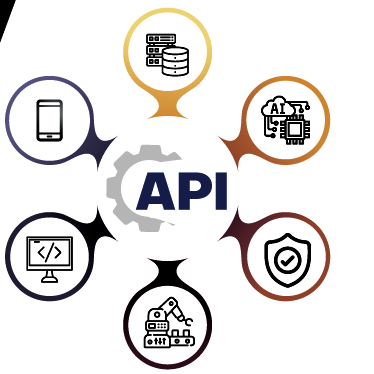
\includegraphics[width=\linewidth]{./images/api_cover.png}
                \caption{Communation among applications.}
            \end{figure}
        \end{column}
    \end{columns}
\end{frame}

\begin{frame}
    \frametitle{Categories of API}
    \begin{enumerate}
        \item Web-based system
        \begin{itemize}
            \item A web API is an interface with a web server.
            \item Extensively used for the development of web applications.
        \end{itemize}
        \item Operating system
        \begin{itemize}
            \item Offers the functionality of various OS features taht can be incorporated in creating windows or mac or linux applications.
        \end{itemize}
        \item Database system
        \begin{itemize}
            \item These APIs are defined in a manner to pass out the requested data in a predefined format that is understandable by the requesting client.
            \item This makes the process of interaction with databases generalised and thereby enhancing the compatibility of applications with the various databases.
        \end{itemize}
    \end{enumerate}
\end{frame}

\begin{frame}
    \frametitle{How Do Web API Work?}
    \begin{columns}
        \begin{column}{0.5\linewidth}
            \begin{figure}
                
\includegraphics[scale=0.12]{./images/api-visual.png}
            \end{figure}
        \end{column}
        \begin{column}{0.5\linewidth}
            \begin{figure}
                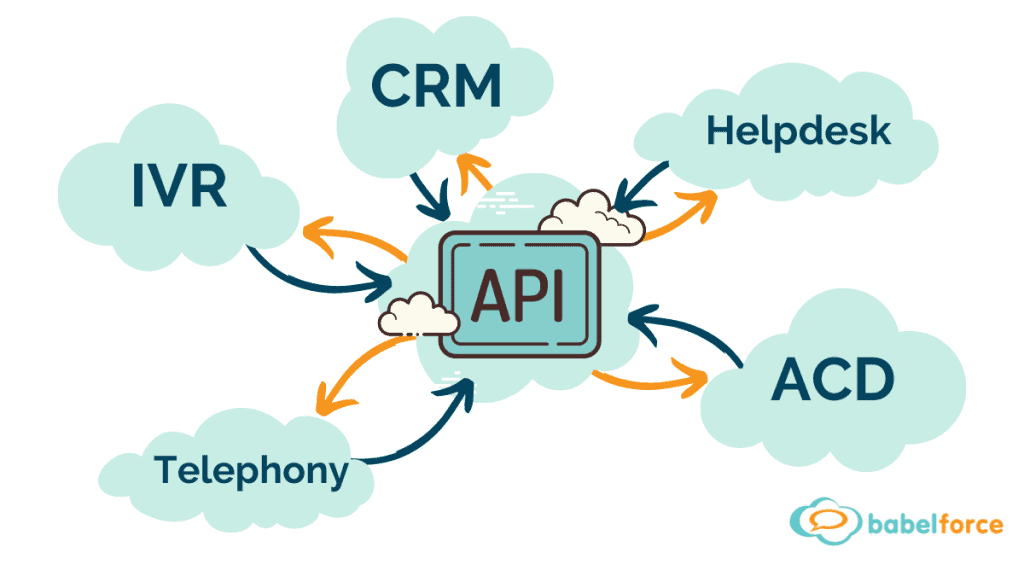
\includegraphics[scale=0.17]{./images/api_internal.png}
            \end{figure}
        \end{column}
    \end{columns}
    \centering
    \text{Figure 2: shows how an API works}
\end{frame}

\begin{frame}
    \frametitle{API in summary}
    \begin{figure}
        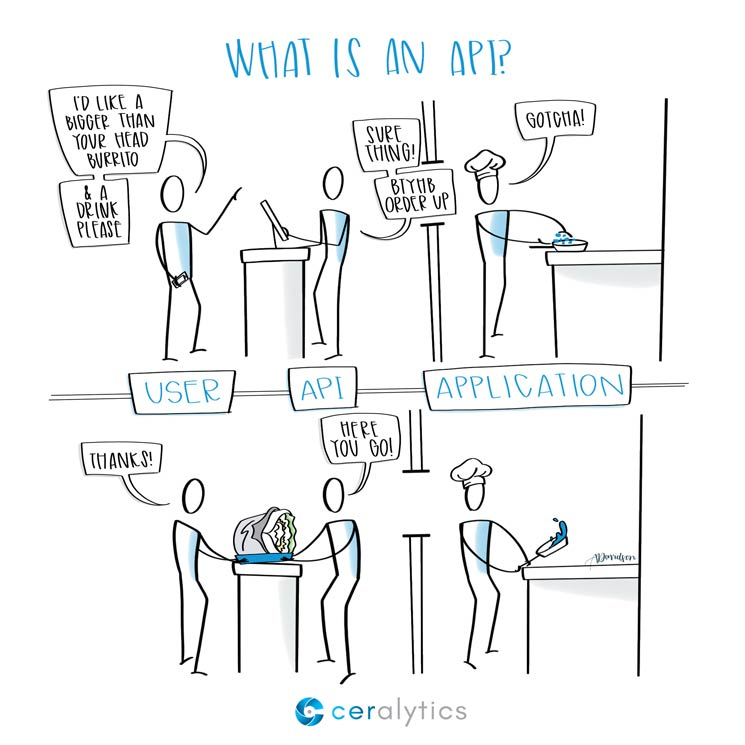
\includegraphics[scale=.25]{./images/what-is-api.jpg}
        \caption{How API works}
        \label{figure:background-story}
    \end{figure}    
\end{frame}

\begin{frame}
    \frametitle{Why do Data Scientists need API?}
    \begin{enumerate}
        \item To access data from external sources, such as databases or web services, in order to integrate that data into their models and analyses. 
        \item To expose models and other tools developed by data scientists to other systems and applications, allowing those systems to make use of the data and insights generated by the data science team
        % \item Share output of your machine learning model (data science project).
        \item To automate certain tasks, such as data collection or model training, which can save time and resources for the data science team.
        % \item API give business access to understandable data that can be used to fuel innovation and growth.
        % \begin{itemize}
        %     \item Helps open up new markets, inspire new business models, and enable business models, enable business partnerships to form.
        % \end{itemize}
    \end{enumerate}
\end{frame}

\begin{frame}
    \frametitle{Examples of API for Data Scientists}
            \begin{enumerate}
                \begin{columns}
                    \begin{column}{0.5\linewidth}
                        \item Amazon Machine Learning API
                        \item IBM Watson Discovery API
                        \item Google API
                        \item Twilio API
                        \item Census.gov API
                        \item Spotify API
                        \item Yummly API          
                    \end{column}
                    \begin{column}{0.5\linewidth}
                        \item Reddit API
                        \item Zillow API
                        \item Instagram API
                        \item Twitter API
                        \item Big ML API
                        \item Data Science Toolkit API 
                        \item New York Times API
                    \end{column}
                \end{columns}
            \end{enumerate}
\end{frame}

\begin{frame}
    \frametitle{How to build a API for Data Sciences}
    \begin{itemize}
        \item Building an API for data science typically involves several steps:
        \begin{enumerate}
            \item Define the API endpoint(s): Determine what data or functionality the API will provide and how it will be accessed (e.g. via a RESTful interface).
            \item Collect and prepare the data: Gather the necessary data and perform any preprocessing or cleaning that is required.
            \item Develop the API: Use a web framework (such as Flask or Django) to develop the API endpoint(s) and connect them to the data.
            \item Test the API: Test the API to ensure it is functioning correctly and providing the expected results.
        \end{enumerate}
    \end{itemize}    
\end{frame}

\begin{frame}
    \frametitle{Con'td}
    \begin{description}
        \item[5] Deploy the API: Deploy the API to a server or hosting platform, making it available for use by other systems and applications.
        \item[6] Secure the API: Implement security measures such as authentication and authorization to protect the API and its data from unauthorized access.
        \item[7] Document the API: Provide clear documentation for the API, including information on how to access it, what data or functionality it provides, and any constraints or limitations.
        \item[8] Monitor and maintain the API: Monitor the API for errors or issues, and make any necessary updates or changes to keep it running smoothly.
    \end{description}
\end{frame}

\begin{frame}
    \frametitle{Demo}
    \textbf{The Architecture and tools}
    \begin{figure}
        \centering
        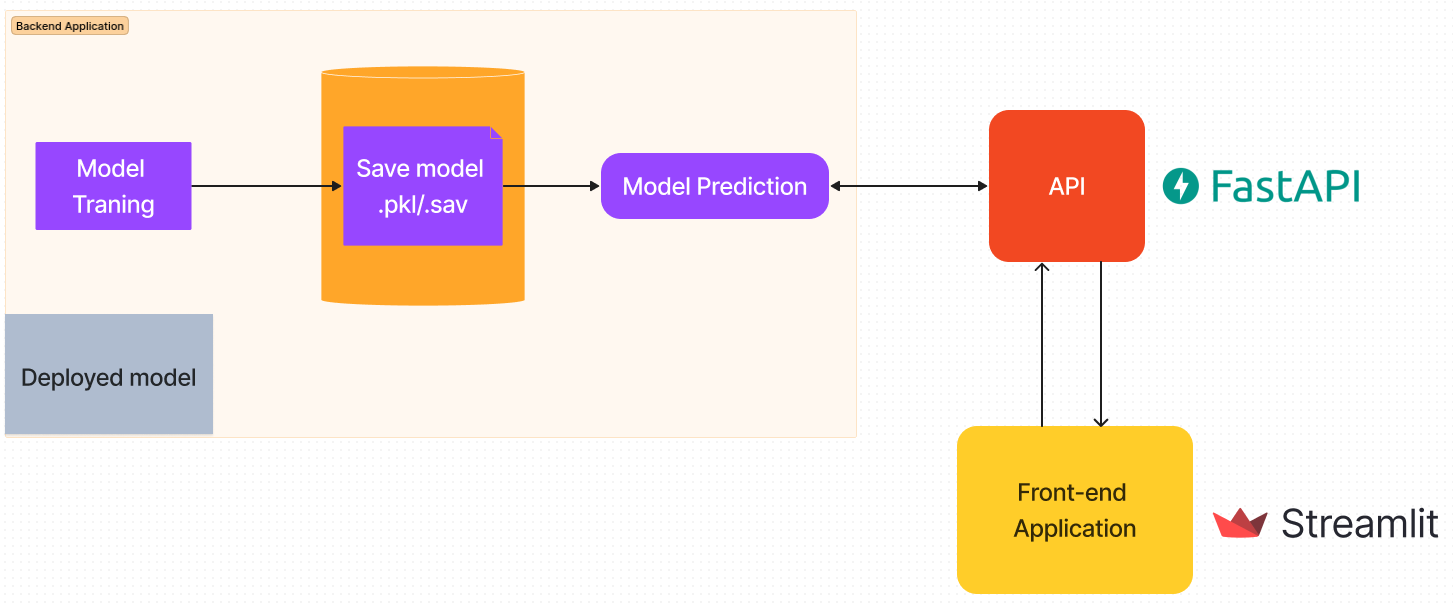
\includegraphics[scale=0.25]{./images/architecture.png}
        \caption{shows the architecture of the demo application}
        \label{figure:architecture}
    \end{figure}
\end{frame}

\begin{frame}
    \centering
    Thank you for your attention.
\end{frame}

\end{document}